


\documentclass[main]{subfiles}

\begin{document}


\chapter{Attributer Class}

\begin{lstlisting}[language=Python,basicstyle=\scriptsize]

import logging

# keras models
from keras.applications import InceptionV3, VGG16, ResNet50
from keras.applications.imagenet_utils import decode_predictions

# util
from eval.util.constants import *
from eval.util.image_util import ImageHandler, show_figure, apply_threshold,
	get_classification_mappings

# methods
from eval.methods.LIME import Lime
from eval.methods.deep_lift import DeepLift
from eval.methods.SHAP import Shap
from eval.methods.grad_cam import GradCam


def check_invalid_attribution(attribution, ih):
    # attribution should be a 2D array returned by each method
    # i.e grayscale not RGB
    if attribution is None:
        return 1
    # check shape of attribution is what is expected
    if attribution.ndim != 2:
        print('Attribution returned has {} dimensions'.format(attribution.ndim))
        return 1
    if attribution.shape != ih.get_size():
        print('Attribution returned with shape {} is not the expected shape of {}'.format(
            attribution.shape, ih.get_size()))
        return 1
    return 0


class Attributer:
    def __init__(self, model_name: str):
        self.models = {
            VGG: VGG16,
            INCEPT: InceptionV3,
            RESNET: ResNet50
        }
        self.curr_model_name = model_name
        self.curr_model = self.load_model(model_name)
        # set up methods
        self.lime_method = None
        self.deep_lift_method = None
        self.shap_method = None
        self.gradcam_method = None
        # Classes for imagenet
        self.class_map = get_classification_mappings()

    def load_model(self, model_name: str):
        self.curr_model_name = model_name
        print('Loading {} model architecture and weights...'.format(model_name))
        return self.models[self.curr_model_name](weights='imagenet')

    def build_model(self):
        """Function returning a new keras model instance.
        """
        if self.curr_model_name == VGG:
            return VGG16(include_top=True, weights='imagenet')
        elif self.curr_model_name == INCEPT:
            return InceptionV3(include_top=True, weights='imagenet')
        elif self.curr_model_name == RESNET:
            return ResNet50(include_top=True, weights='imagenet')

    def initialise_for_method(self, method_name: str, layer_no: int = None):
        if method_name == LIFT and self.deep_lift_method is None:
            self.deep_lift_method = DeepLift(self.curr_model, self.build_model)
        elif method_name == LIME and self.lime_method is None:
            self.lime_method = Lime(self.curr_model, self.curr_model_name)
        elif method_name == SHAP and self.shap_method is None:
            print(layer_no)
            self.shap_method = Shap(self.curr_model, self.curr_model_name, 
                                    layer_no)
        elif method_name == GRAD and self.gradcam_method is None:
            self.gradcam_method = GradCam(self.curr_model, self.build_model, 
                                          layer_no)

    def predict_for_model(self, ih: ImageHandler, top_n: int = 5, 
                          print_to_stdout: bool = True) -> (str, float):
        # returns a tuple with the top prediction, and the probability of the 
        # top prediction (i.e confidence)
        logging.info('Classifying...')
        predictions = self.curr_model.predict(ih.get_processed_img())
        decoded_predictions = decode_predictions(predictions, top=top_n)

        # print the top 5 predictions, labels and probabilities
        if print_to_stdout:
            print('Model predictions:')
        max_p = 0.00
        max_pred = ''
        for (i, (img_net_ID, label, p)) in enumerate(decoded_predictions[0]):
            if print_to_stdout:
                print('{}: {}, Probability={:.2f}, ImageNet ID={}'.format(
                    i + 1, label, p, img_net_ID))
            if p > max_p:
                max_p = p
                max_pred = label
        if print_to_stdout:
            print('')
        return max_pred, max_p

    def get_good_examples(self, cap: int = 1001):
        good_examples = []
        for i in range(1, cap):
            ih = ImageHandler(i, self.curr_model_name)
            max_pred, p = self.predict_for_model(ih, top_n=1, 
                                                 print_to_stdout=False)
            if p > 0.9:
                good_examples.append(i)
        return good_examples

	\end{lstlisting}        
	\newpage
	\begin{lstlisting}[language=Python,basicstyle=\scriptsize]
        
    def attribute(self, ih: ImageHandler, method: str, layer_no: int = None,
                  take_absolute: bool = False, take_threshold: bool = False, 
                  sigma_multiple: int = 0,
                  visualise: bool = False, save: bool = True):
        if layer_no is None:
            layer_no = LAYER_TARGETS[method][self.curr_model_name]
        self.initialise_for_method(method_name=method, layer_no=layer_no)
        # get the 2D numpy array which represents the attribution
        attribution = self.collect_attribution(ih, method=method, layer_no=layer_no)
        # check if applying any thresholds / adjustments based on +ve / -ve evidence
        if take_threshold or take_absolute:
            attribution = apply_threshold(attribution, sigma_multiple, 
                                          take_absolute)
        if check_invalid_attribution(attribution, ih):
            return
        if save:
            ih.save_figure(attribution, method)
        if visualise:
            show_figure(attribution)
        return attribution

    def attribute_panel(self, ih: ImageHandler, methods: list = METHODS,
                        take_threshold: bool = False, sigma_multiple: int = 0, 
                        take_absolute: bool = False,
                        visualise: bool = False, save: bool = True):
        output_attributions = {}
        for method in methods:
            layer_no = LAYER_TARGETS[method][self.curr_model_name]
            output_attributions[method] = self.attribute(ih=ih, method=method, 
                                                         layer_no=layer_no,
                                                         take_absolute=take_absolute, 
                                                         take_threshold=take_threshold,
                                                         sigma_multiple=sigma_multiple,
                                                         visualise=visualise, save=save)
        return output_attributions

    def collect_attribution(self, ih: ImageHandler, method: str, 
                            layer_no: int = None, print_debug: bool = True):
        """Top level wrapper for collecting attributions from each method. """
        if print_debug:
            print('Collecting attribution for `{}`'.format(method))
        if method == LIFT:
            return self.deep_lift_method.attribute(ih)
        elif method == LIME:
            return self.lime_method.attribute(ih)
        elif method == SHAP:
            self.shap_method.reset_explainer(layer_no=layer_no)
            return self.shap_method.attribute(ih)
        elif method == GRAD:
            self.gradcam_method.reset_layer_no(layer_no=layer_no)
            return self.gradcam_method.attribute(ih)
        else:
            print('Error: Invalid attribution method chosen')
            return None


\end{lstlisting}

\newpage
\chapter{Evaluator Class}

\begin{lstlisting}[language=Python,basicstyle=\scriptsize]

import os
import pandas as pd
import numpy as np

# Attributer class
from eval.Attributer import Attributer

# util
from eval.util.constants import *
from eval.util.image_util import ImageHandler, show_figure, 
	show_intersect_union_subfigures
from eval.util.imagenet_annotator import get_mask_for_eval


class Evaluator:
    def __init__(self, metric: str, model_name: str, att: Attributer = None):
        if att is None:
            self.att = Attributer(model_name=model_name)
        else:
            self.att = att
        self.metric = metric
        self.model_name = model_name
        self.file_headers = METHODS  # [m + "+_" + self.model_name for m in METHODS]
        self.result_file = "{}/{}/{}_results.csv".format(
            RESULTS_EVAL_PATH, model_name, metric)
        self.results_df = self.read_file(self.result_file, wipe=False)

    def read_file(self, file_path: str, wipe=False):
        # gets a dataframe from the results file
        if wipe:
            f = open(file_path, "w+")
            f.close()
            df = pd.DataFrame(columns=['img_no'] + self.file_headers).set_index(
                'img_no')
            return df
        if not os.path.exists(file_path):
            with open(file_path, "w") as f:
                f.write(','.join(['img_no'] + self.file_headers))
        df = pd.read_csv(file_path).set_index('img_no')
        return df

    def write_results_to_file(self):
        self.results_df.to_csv(self.result_file, index=True, index_label='img_no')

    def get_image_handler_and_mask(self, img_no):
        # this gets the image wrapped in the ImageHandler object, and the 
        # bounding box annotation mask for the image,
        # ImageHandler is used to calculate attributions by each method, and the
        # mask is used for evaluation
        ih = ImageHandler(img_no=img_no, model_name=self.model_name)
        # bounding box in the format of the model's input shape / attribution shape
        annotation_mask = get_mask_for_eval(img_no=img_no, target_size=ih.get_size(),
                                            save=False, visualise=False)
        return ih, annotation_mask

    def collect_panel_result_batch(self, experiment_range: list):
        new_rows = {}
        for img_no in experiment_range:
            new_row = {}
            ih, annotation_mask = self.get_image_handler_and_mask(img_no)
            for method in METHODS:
                result = self.collect_result(ih, annotation_mask, method)
                if img_no <= len(self.results_df.index):
                    self.results_df.at[img_no, method] = result
                else:
                    new_row[method] = result
            new_rows[img_no] = new_row
            if (img_no % 10) == 0:
                self.append_to_results_df(new_rows)
                new_rows = {}
        self.append_to_results_df(new_rows)

    def collect_result_batch(self, method: str, experiment_range: range):
        new_rows = {}
        for img_no in experiment_range:
            ih, annotation_mask = self.get_image_handler_and_mask(img_no)
            result = self.collect_result(ih, annotation_mask, method)
            if img_no <= len(self.results_df.index):
                self.results_df.at[img_no, method] = result
            else:
                new_rows[img_no] = {method: result}
            if img_no % 10 == 0:
                self.append_to_results_df(new_rows)
                new_rows = {}

        self.append_to_results_df(new_rows)

    def append_to_results_df(self, new_rows_dict, write=True):
        new_data = pd.DataFrame.from_dict(new_rows_dict, 
                                          columns=self.file_headers, 
                                          orient='index')
        self.results_df = self.results_df.append(new_data, sort=True)
        if write:
            self.write_results_to_file()

    def collect_result(self, ih: ImageHandler, mask, method: str):
        # threshold for each attribution's "explainability" is the number of std 
        # deviations above the mean contribution score for a pixel
        if self.metric == INTERSECT:
            return self.evaluate_intersection(ih, mask, method, 
                                              sigma=INTERSECT_THRESHOLD)
        elif self.metric == INTENSITY:
            return self.evaluate_intensity(ih, mask, method, 
                                           sigma=INTENSITY_THRESHOLD)

    def evaluate_intersection(self, ih: ImageHandler, mask, method: str, 
                              sigma: int, print_debug: bool = False) -> float:
        # calculate an attribution and use a provided bounding box mask to 
        # calculate the IOU metric. attribution has threshold applied, and abs 
        # value set (positive and negative evidence treated the same)
        attribution = self.att.attribute(ih=ih,
                                         method=method,
                                         layer_no=LAYER_TARGETS[method][self.model_name],
                                         take_threshold=True, sigma_multiple=sigma, 
                                         take_absolute=True,
                                         visualise=False, save=False)
        # calculate the intersection of the attribution and the bounding box mask
        intersect_array = np.zeros(attribution.shape)
        intersect_array[(attribution > 0.0) * (mask > 0.0)] = 1
        # get the union array for the IOU calculation
        union_array = np.zeros(attribution.shape)
        union_array[(attribution > 0.0) + (mask > 0.0)] = 1
        # calculate intersection and union areas for numerator and 
        # denominator respectively
        intersect_area = intersect_array.sum()
        union_area = union_array.sum()
        intersection_over_union = intersect_area / union_area
        print('Evaluating `{}` on example `{}` ({})'.format(
            method, ih.img_no, 'intersection'))
        if print_debug:
            #print('--Mask Area =\t {}'.format(mask_area))
            print('--Intersect Area =\t {}'.format(intersect_area))
            print('--Union Area =\t {}'.format(union_area))
            print('--Intersection / Union =\t{:.2f}%'.format
                  (intersection_over_union * 100))
            print('')

        return intersection_over_union

    def evaluate_intensity(self, ih: ImageHandler, mask, method: str, sigma: int, 
                           print_debug: bool = False) -> float:
        # # calculate an attribution and use a provided bounding box mask to 
        # calculate the IOU metric attribution has threshold applied, and abs 
        # value set (positive and negative evidence treated the same)
        attribution = self.att.attribute(ih=ih,
                                         method=method,
                                         layer_no=LAYER_TARGETS[method][self.model_name],
                                         take_threshold=True, sigma_multiple=sigma, 
                                         take_absolute=True,
                                         visualise=False, save=True)
        # calculate the weight/confidence of the attribution intersected with 
        # the bounding box mask
        intensity_array = np.copy(attribution)
        intensity_array[(attribution > 0.0) * (mask < 0.1)] = 0
        # get the union array for the IOU* calculation
        union_array = np.zeros(attribution.shape)
        union_array[(attribution > 0.0) + (mask > 0.0)] = 1
        intensity_area = intensity_array.sum()
        union_area = union_array.sum()
        intensity_over_union = intensity_area / union_area
        print('Evaluating `{}` on example `{}` ({})'.format(
            method, ih.img_no, 'intensity'))
        if print_debug:
            print('--Intersect Area =\t {}'.format(intensity_area))
            print('--Union Area =\t {}'.format(union_area))
            print('--Intensity / Union =\t{:.2f}%'.format(intensity_over_union * 100))
            print('')

        return intensity_over_union



\end{lstlisting}


\chapter{VGG16 Supportive Results}

Supportive results for Section \ref{sec:vggExp}. These results are from a smaller experiment run on VGG16 with a different threshold set: 1 std dev. for IOU and 2 for IOU*.

%\vspace{2in}

\begin{figure}[h]\centering
\vfill
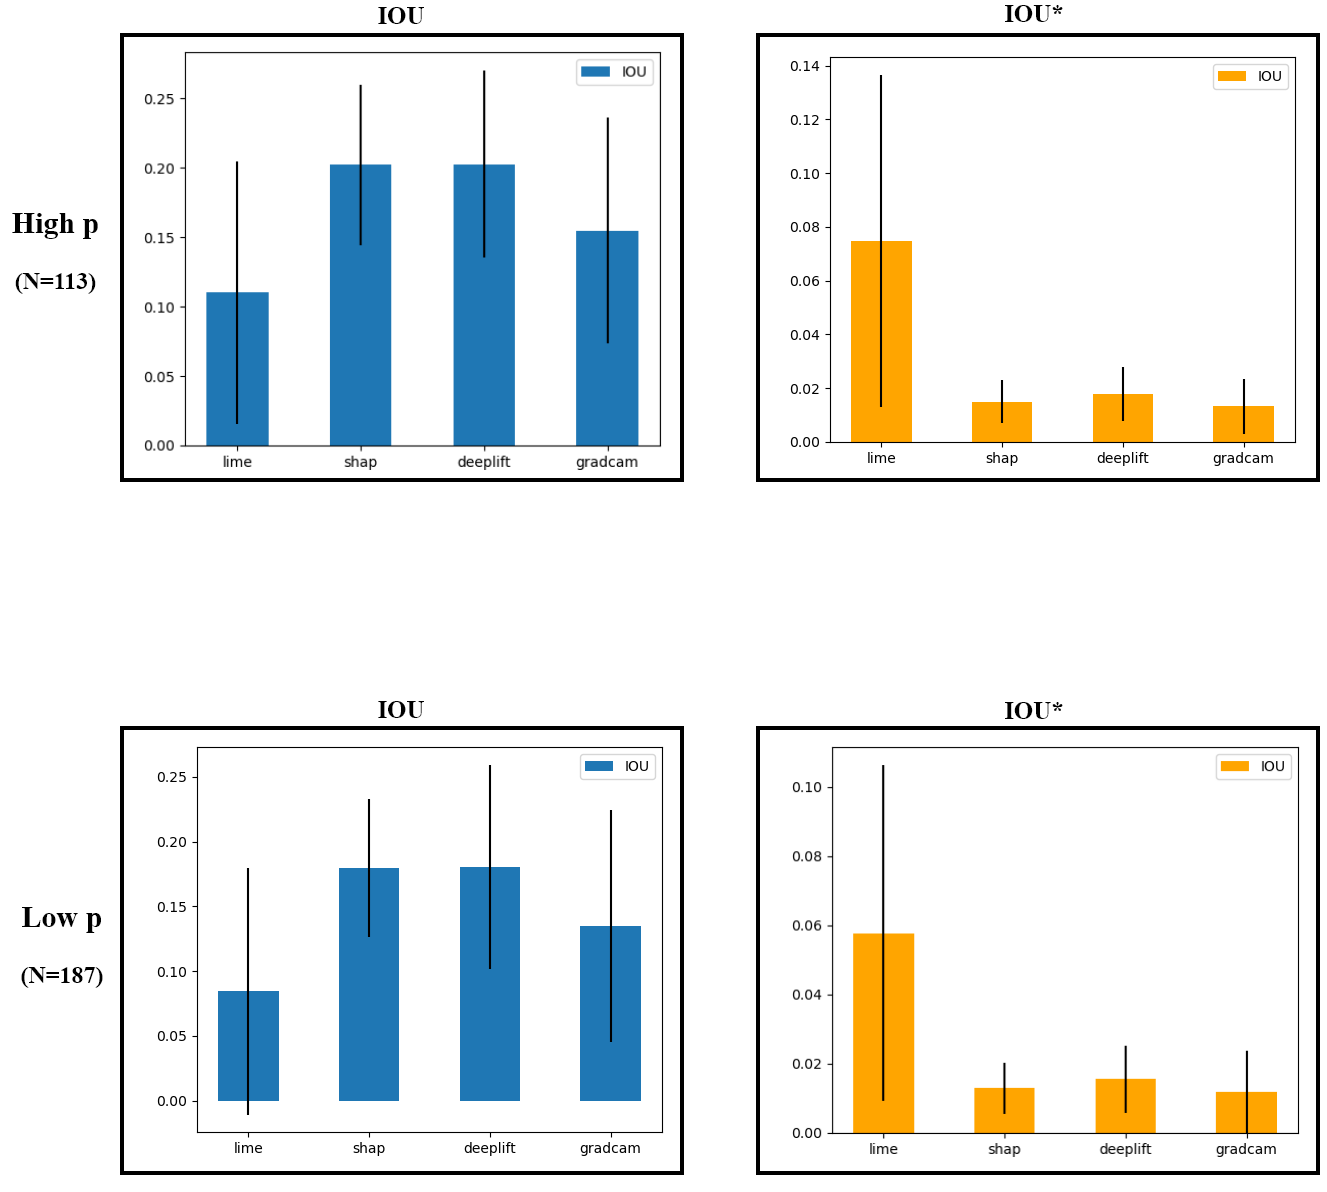
\includegraphics[scale=0.30]{appendix_C.png}
\caption{Results for a 300-instance attribution sample of VGG16. }
\label{vggExtraFig}
\vfill
\end{figure}


\end{document}